\chapter{Реализация клиент-серверного взаимодействия по протоколу WebSocket}

\section{Пример простого чата (node.js)}

Рассмотрим пример приложения, созданного на node.js.

Сервер запускается на порту 8080, и ожидает подключения клиента (листинг 2.1). В данном случае мы не обеспечиваем никакого шифрования и должной обработки ошибок, наша задача просто продемонстрировать принцип работы.

\lstinputlisting[language=JavaScript, caption={Исходный код сервера node.js приложения}]
{example1/server.js}

Как только клиент подключился, сервер отдаёт ему HTML страницу с кодом на JavaScript. Этот выполняет WebSocket подключение к серверу для обмена сообщениями (листинг 2.2).

\lstinputlisting[language=HTML, caption={Исходный код клиента}]
{example1/index.html}

Если открыть это соединение из двух разных браузеров, можно устроить простой чат (рисунок 2.1).

\begin{figure}[H]
\centering
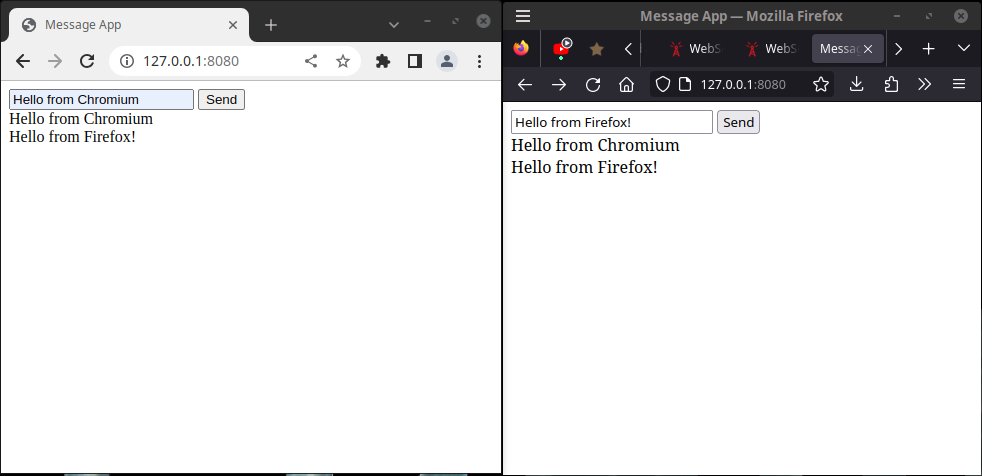
\includegraphics[scale=0.5]{res/browsers1}
\caption{Взаимодействие между двумя разными браузерами}
\end{figure}

В это время в терминале можно видеть сообщения, которыми обмениваются клиенты (рисунок 2.2).

\begin{figure}[H]
\centering
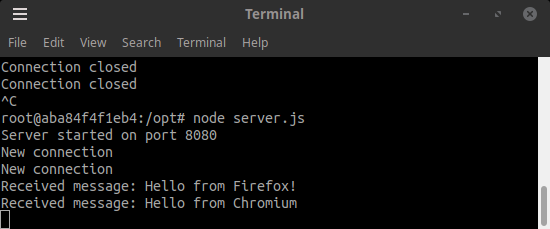
\includegraphics[scale=1]{res/console1}
\caption{Консоль серверного приложения}
\end{figure}

\section{Пример тестера скорости соединения (Rust)}

Второй пример представляет из себя немного более сложный код. Идея проекта в том, чтобы передать через WebSocket соединение файл объёмом 10 мб и замерить скорость передачи.

Сервер так же запускается на порту 8080 (листинг 2.3), и готов отдать пользователю статичный HTML файл.

\lstinputlisting[language=Rust, caption={Исходный код сервера Rust приложения}]
{example2/src/main.rs}

Управление раутами и временем жизни соединения в этот раз вынесено в отдельный файл (листинг 2.4)

\lstinputlisting[language=Rust, caption={Управление WebSocket соединением}]
{example2/src/server.rs}

Клиентское приложение представляет из себя HTML страницу (листинг 2.5). Её код тривиален, поэтому в листинге обратим внимание только на JavaScript код.

\lstinputlisting[language=JavaScript, caption={Исходный код сервера node.js приложения}, , firstline=83, lastline=175]
{example2/static/index.html}

В панели веб-разработчика можно видеть, что файл действительно был передан именно через WebSocket (рисунок 2.3).

\begin{figure}[H]
\centering
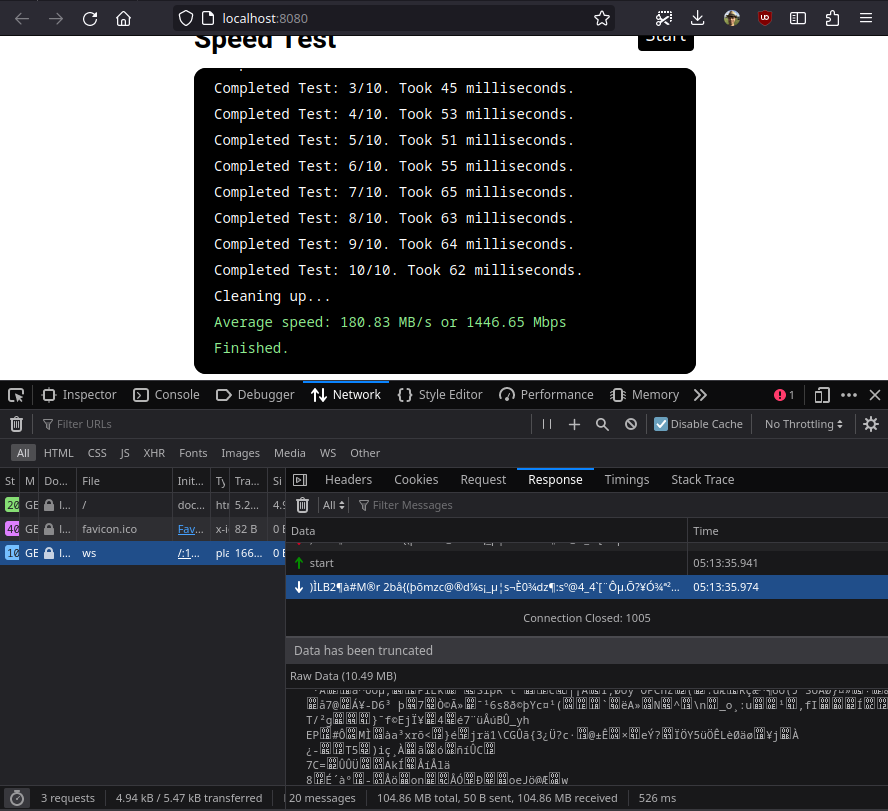
\includegraphics[scale=0.6]{res/browser2}
\caption{Панель веб-разработчика}
\end{figure}
